

This chapter provides a description of the OCEAn application.
This includes implementation details and information on the libraries used (\autoref{sec:impl-architecture})
and a typical user journey (\autoref{sec:impl-journey}).


% ---------------------------------------------------------------------
% ---------------------------------------------------------------------
\section{Architecture}
\label{sec:impl-architecture}
% ---------------------------------------------------------------------
% ---------------------------------------------------------------------

The OCEAn application is a web-based program consisting of two parts:
A python backend for importing and exporting OCEL files and executing all computations for emission estimation and object allocation,
and a TypeScript~\cite{TypeScript} frontend based on
React\footnote{\url{https://react.dev/}}.

The backend provides a wrapper class for pm4py~\cite{Berti23pm4py} OCELs offering various statistics and transformations, such as the discovery of object interactions for building the object interaction graph.

The frontend accesses backend functions by means of an API developed with
FastAPI\footnote{\url{https://fastapi.tiangolo.com/}}.
This library offers data validation based on
pydantic~\cite{pydantic24}
and thus ensures type safety in all parameters passed through the API. Additional sanity checks are integrated as custom pydantic validators and assertions.

The application is designed to handle large datasets.
All computations involving OCEL data are implemented using vectorized operations with the \texttt{pandas}~\cite{pandas24,McKinney10pandas} package.
% and \texttt{numpy} packages.
As the OCEL import is potentially a long-running, the imported OCEL is always kept in server memory during a session. This makes the API stateful, allowing for further performance optimizations. Caching is used for repeated calls to the same function. To enable caching for functions with list or set parameters, the
\texttt{cachetools}~\footnote{\url{https://github.com/tkem/cachetools/}}
library is used, facilitating customization of function argument hashing as opposed to python's built-in caching functionality.
% For long-running tasks like the \allocrule{ClosestTargets} object allocation, the backend is designed

Allocation graphs are handled using \texttt{networkx}~\cite{Hagberg08networkx} data structures.
However, as the distance computation for the \allocrule{ClosestTargets} rule requires finding not only one, but all closest target objects, a custom BFS implementation is used, as stated in \autoref{fig:eva-setup}.

The OCEAn application is publicly accessible on GitHub~\footnote{\url{https://github.com/rwth-pads/ocean}}.

% ---------------------------------------------------------------------
% ---------------------------------------------------------------------
\section{User Journey}
\label{sec:impl-journey}
% ---------------------------------------------------------------------
% ---------------------------------------------------------------------

When opening the application, the user is first offered a file upload for event logs in the OCEL~2.0 sqlite format.
Alternatively, some example logs are provided for quick access, including the logistics example OCEL from \autoref{ssec:prelim-ocel-rex} and four OCELs later used for evaluation (\autoref{chap:eva}).

After loading an OCEL into the application, the main dashboard (\autoref{fig:app-screen-overview}) is shown. The page consists of multiple sections:
The \textit{Overview} section contains basic information about the dataset, including the number of events and objects and its filename. Additional metadata like a source URL can be included here.

\begin{figure}[t]
  \begin{small}
    \begin{center}
      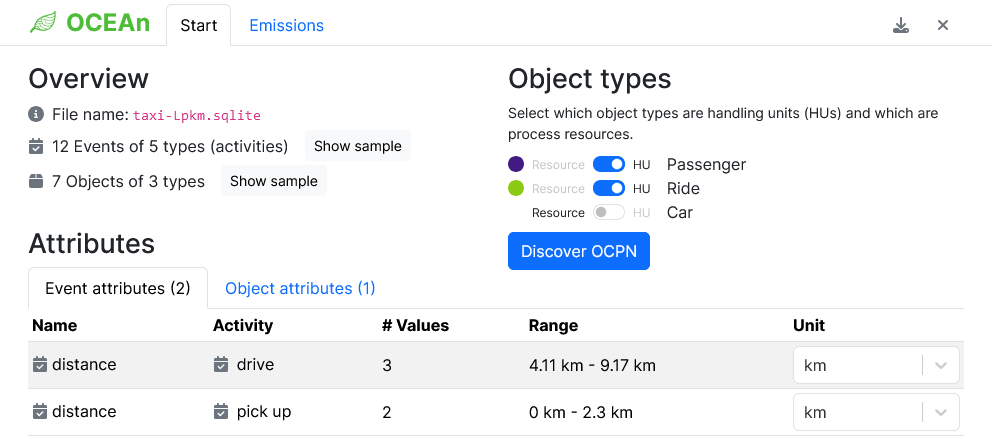
\includegraphics[width=\textwidth]{figures/screenshots/20240901-ocean-overview1.png}
    \end{center}
    \caption{Dashboard of the OCEAn app. On the top left, basic information about the OCEL is shown. On the bottom, the available attributes are listed and assigned a unit. On the top right, the HU/resource partition is defined.}
    \label{fig:app-screen-overview}
  \end{small}
\end{figure}

In the \textit{Attributes} section, the event and object attributes contained in the OCEL are listed. Basic statistics such as number of distinct values of categorical attributes and minimum and maximum of numerical attributes are offered. For numerical attributes, a unit selection is available. As OCELs do not natively contain information about the unit of quantities represented as attributes, this has to be added manually by the user.
This enables automatic unit conversion when applying emission rules. To this end, the \texttt{pint} python library is employed.
When defining emission rules, a sanity check is performed to ensure the multiplication result is always a weight (e.g., \unit{\kgcotwoe}), prohibiting erroneous selection of attributes or units.

The \textit{Object types} section offers controls to partition the object types into sets of HUs and resources. This is necessary in order to configure the \allocrule{ClosestTargets} rule for object allocation.
Object types are always displayed with an icon that is colored in different hues for HUs and gray for resources. HU colors are automatically generated every time the set of HUs changes. Colors are generated with hues distributed equidistantly and randomized brightness and saturation values.

\begin{figure}[t]
  \begin{small}
    \begin{center}
      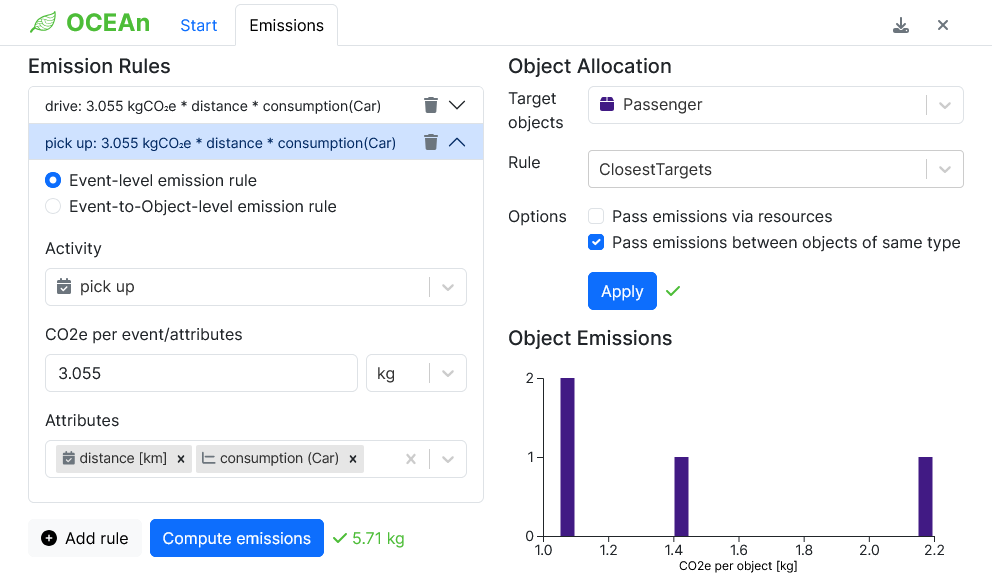
\includegraphics[width=\textwidth]{figures/screenshots/20240901-ocean-emissions.png}
    \end{center}
    \caption{Emissions page of the OCEAn app. On the left, emission rules are defined specifying an activity and an emission factor linked to attributes. On the right, object allocation parameters are controlled. Below, the resulting target object emissions are shown in a histogram.}
    \label{fig:app-screen-emissions}
  \end{small}
\end{figure}

In the header, the \textit{Emissions} tab can be accessed. Also, a download button allows exporting the OCEL with newly integrated data.
In case emission data has already been computed on both event and object level,
the user is prompted on what level to include these data.
This is because the overall emission sum has to be conserved.
Apart from event emissions, the export includes all user inputs made in the app, like attribute units, emission rules and the HU/resource partition.
These data are integrated into the OCEL~2.0 \texttt{sqlite} file by adding an additional table. When importing an OCEL, the settings are loaded in order to increase usability and session portability.

The \textit{Emissions} tab (\autoref{fig:app-screen-emissions}) includes an interface for adding and editing emission rules. Both event and E2O emission rules are supported. An activity (and object type and qualifier in the case of E2O rules) is selected and an emission factor is introduced. The user can select one or multiple attributes linked to the respective activity or its unique object types.
After emission computation is triggered, the overall emissions are shown to the user.

As soon as emission data are available, the object allocation interface is shown on the right side. Here, all parameters like the allocation rule and additional configuration of the \allocrule{ClosestTargets} rule are set. Target objects can be chosen, with the selection limited to object types for usability reasons. In practice, this means that $\Omega=\{ o\in O \mid \objtype(o)=\ot \}$ for the selected object type $\ot\in\OTL$.
After running allocation, the resulting object emission distribution is shown in a histogram.

